\section{Experiment}
\label{sec:experiments}

The present experiment investigates whether different, syntax-based classes of compound words (Subordinate, Attributive, and Coordinate) can be captured by means of semantic properties of the compound and its constituents. To quantify these properties, (a) we generate compositional representations of compounds and obtain similarity scores assessing the role of each constituent in contributing to the overall meaning; (b) we measure the degree of similarity between the first and second constituent.

A note on the terminology used in the paper. Until this point, we used the neutral terms `first constituent' and `second constituent' to refer to, respectively, \emph{dog} and \emph{house} in \emph{doghouse}. As briefly mentioned in section \ref{sec:class}, one constituent usually plays a dominant role compared to the other since it acts as the `head' of underlying phrase. In this example, the head is clearly \emph{house} (indeed, \emph{doghouse} is `the house of the dog'). Consistently, this element determines the syntactic category of the phrase and, semantically, it represents a hyperonym of the compound. By default, in English compounds the second constituent acts as the compound `head', whereas the first acts as the compound `modifier' \citep{bauerOHC}. We stick with this arguably simplified terminology\footnote{Without going into much detail, it should be mentioned that this picture is indeed less straightforward than it may appear. For instance, in the English compound \emph{singer-songwriter} the two constituents play a similar role, in a way that they could be both considered as the compound `head' (and the compound as `double-headed') \citep{bauerOHC}} and, from now on, we interchangeably use the terms `first constituent' or `modifier' to refer to the leftmost element, `second constituent' or `head' to refer to the rightmost one.


\subsection{Semantic space}\label{sec:vectors}

Following \cite{baronipredict}, who demonstrated that DSMs generated using feedforward neural networks models largely outperform traditional count-based architectures in many tasks, we built a state-of-the-art \texttt{CBOW} semantic space using the \texttt{word2vec} toolkit by \cite{mikolov2013}, with all the parameters that turned out to be best-predictive in \cite{baronipredict}. In particular, the vectors have 400 dimensions and were built using (a) a context window of 5 words to either side of the target word, (b) a subsampling procedure which penalizes high-frequency words in the training phase (t = 1e\textsuperscript{-5}), (c) 10 negative samples. The vectors were trained using a corpus of written English containing around 2.8-billion tokens (a concatenation of BNC, ukWaC, and a 2009-dump of Wikipedia), the same used in \cite{baronipredict}. To avoid sparsity effects, we experimented with the vectors corresponding to the 300K most frequent words in the corpus.


\subsection{Materials}

We experimented with a sample of the MorBoComp database including 163 English compounds. MorboComp is a large, multilingual database of compounds that has been developed to study compounding from a typological perspective.\footnote{For further details, see: \url{http://morbocomp.sslmit.unibo.it/index.php?section=home}} Each compound in the database is richly annotated (i.e., it is provided with information about headedness, compound and constituents' grammatical category, compound structure, etc.) and, crucially for our purposes, it is classified as Subordinate (hence, SUB), Attributive (hence, ATT) or Coordinate (hence, CRD) on the basis of the classification and terminology proposed by \cite{SB2005}. To illustrate, \emph{schoolteacher} is tagged as SUB, \emph{keyword} as ATT, and \emph{king-emperor} as CRD.

Consistently with the criteria outlined in \cite{SB2005}, the 163-item sample contained cases of both `phrasal' compounds (\emph{do-it-yourself illustration}, \emph{around-the-world flight}) and `neoclassical' formations (\emph{bibliography}, \emph{theology}). In addition, a handful of items labeled with OTH (i.e., Other) were found. Since this label was used by the annotators for either unresolved or idiosyncratic cases, however, we decided not to consider them in our investigation. Similarly, we removed neoclassical formations since their constituents can be affixes and suffixes rather than free-standing, independent words (e.g. \emph{biblio-}). As a consequence, in our distributional semantics approach we could not have a vector representation for these items. Finally, additional 9 compounds were discarded since one of their constituents turned out not to be included in the 300K-vector semantic space. Specifically, 8 out of 9 of the missing items were first constituents of phrasal compounds, e.g. \emph{all-goes-well} (\emph{in all-goes-well atmosphere}) or \emph{floor-of-a-birdcage} (\emph{in floor-of-a-birdcage taste}), whereas in one case (\emph{well-deserver}) the missing items was the second constituent (\emph{deserver}). After this filtering process, our resulting dataset included 132 compounds (67 SUB, 49 ATT, 16 CRD), that we used for our experiment.


\subsection{Generating composed representations}


For each of the 132 compounds in the list, we generated a composed representation using the vectors described in section \ref{sec:vectors} and the compositional model by \cite{guevara2010}. As previously mentioned, one of the main strengths of compositional DSMs is their ability to produce meaning representations also for combinations that are not attested in the source corpus. That is, given a novel or unattested compound, we are able to represent it as an independent vector on the basis of the meanings of its constituents (\emph{zebra} and \emph{horse}). This aspect was of crucial importance in our experiment, where 60 out of the 132 compounds extracted from MorBoComp turned out not to be present in the source semantic space. That is, almost half of the compounds were not among the 300K most frequent words in the corpus and, consequently, did not have a distributional representation. By using a compositional model capitalizing on the representations of the two constituents, however, we were able to overcome this limitation of traditional DSMs and generate a meaning representation for all the items, regardless of whether they had a `static' semantic representation or not.



The method used in the present study, in particular, was implemented by \cite{guevara2010} to model compositionality as depending on the semantic relation instantiated in the syntactic structure. As such, it looks particularly suitable for the case of compounds, which embed a modifier-head structure. Indeed, previous work proved this model to be very effective in generating composed representations for compounds \citep{marelli2017}. Technically, the composed representations are obtained with the combinatorial procedure depicted in Figure~\ref{fig:caoss}: given two vectors \(\vec{u}\) and \(\vec{v}\) each representing one of the constituent words, their composed representation can be computed as \(\vec{c}\) = \textbf{M}\(\vec{u}\) + \textbf{H}\(\vec{v}\), where \textbf{M} and \textbf{H} are weight matrices estimated from training examples. These matrices are trained using least squares regression,\footnote{As reported by \cite{guevara2010}, this method is commonly employed to approximate functions in problems of multivariate multiple regression with a small number of observations and a greater number of variables, that is a similar condition to the one involving high-dimensionality vectors representing word meanings and (relatively) limited data.} having the vectors of the constituents as independent words (\textit{dog}, \textit{house}) as inputs and the vectors of example compounds (\textit{doghouse}) as outputs. The two matrices are thus optimized so that the similarity between the weighted sum of the two constituent vectors (the composed vector) and the compound vector extracted from the semantic space (the observed vector) is maximized. Or, in other words, the composed vector obtained by means of the compositional model is built in a way that closely approximates the original one.


\begin{figure}[t!]
\begin{center}
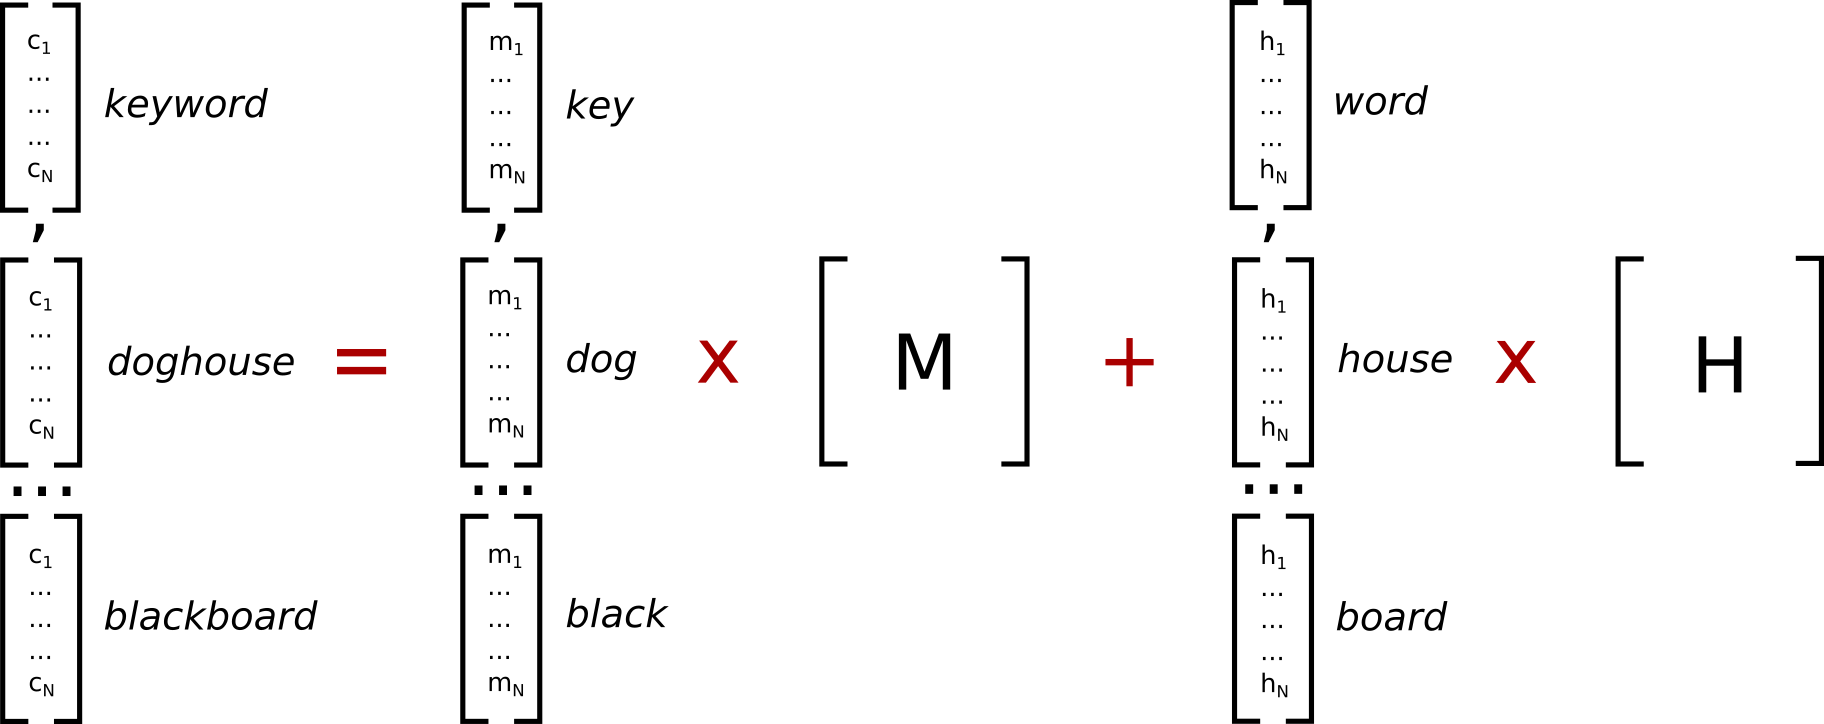
\includegraphics[width=0.9\textwidth]{figures/plsr1.png}
\caption{Representation of the training phase of the compositional method used in the study (adapted from~\citealt{marelli2017}).}\label{fig:caoss}
\end{center}
\end{figure}




In the present study, we trained the compositional model with a list of English noun-noun compounds extracted from the CELEX English Lexical Database \citep{celex}. By default, we treated all compounds as written in \emph{solid} form, that is, without whitespaces or hyphens between the two constituents. When the solid compound was not found in our semantic space, we looked for it in its hyphenated form. The training set included 2174 triplets <modifier, head, compound>, none of which was also present in the dataset we obtained from MorBoComp. We then used the estimated weight matrices for generating composed representations for each of the 132 compounds in our sample.


\subsection{Semantic variables}

For each vector obtained compositionally, we computed four composition-based semantic measures, namely (1) similarity between the composed representation of the compound and its modifier (e.g. between \emph{keyword} and \emph{key}), (2) similarity between the composed representation of the compound and its head (e.g. between \emph{keyword} and \emph{word}), (3) neighborhood density, that is, the average cosine similarity between the composed vector and its top-10 nearest neighbor vectors in the semantic space (all these 3 measures have been introduced by \citealt{vecchi2011}), and (4) entropy, that is a measure of vector quality firstly introduced by \cite{lazaridoufish}.

By operationalizing the similarity between the composed compound vector and either constituents, in particular, we aimed at quantifying the extent to which each single word contributes to the overall, compositionally-obtained meaning. Although operationalized in terms of the cosine of the angle between the compound vector and either constituents (in the same way as standard DSMs do), indeed, these measures genuinely describe the morphological process itself rather than merely taking into account its starting and ending points. Based on these properties, such measures have been recently used in studies with compound words. For example, they have been shown to be effective in predicting meaningfulness ratings on novel combinations \citep{gunther2016} and in capturing relational information in compounds \citep{marelli2017}.

As far as neighborhood density and entropy are concerned, both of them have been proposed to provide information about the meaningfulness of vectors encoding new concepts. The rationale of the former is that meaningful vectors should live in a region of the semantic space that is densely populated by vectors representing many related concepts, while meaningless vectors should be way more isolated. For the latter, the intuition is that meaningful vectors should have a skewed distribution, with few dimensions (corresponding to the salient semantic features of the word) being highly activated, namely having large values. In contrast, meaningless vectors should have a more uniform distribution, which would be a proxy for a less defined, fuzzier meaning. As a consequence, entropy would be inversely correlated with meaningfulness.

A (5) fifth semantic but non-compositional measure was introduced following \cite{lynott2001}, who employed Latent Semantic Analysis (LSA) to quantify the degree of similarity between the first and the second constituent of a compound. Here, we took the compound constituent vectors (e.g. the vectors of \emph{key} and \emph{word}) from the source semantic space (see section~\ref{sec:vectors}) and simply computed their cosine similarity. This measure might be helpful in distinguishing between different compound classes, based on the evidence that in both theoretical linguistics (see \citealt{lieber5OHC}) and conceptual combination literature (see \citealt{wisniewski1996}) this factor has been considered as explanatory of different classes/interpretations.

\subsection{Non-semantic variables}

In addition to the 5 semantic variables described above, we also included in our experiment a number of non-semantic control variables. For each compound and its constituent words we extracted word-form frequency from the source corpus (i.e., the number of times a word is encountered in the corpus in that exact form, regardless of its grammatical category). Compound frequency was calculated by summing the occurrences of the given compound in both solid and hyphenated orthographic form (\emph{blackboard} and \emph{black-board}, respectively). All frequency values, namely (6) compound frequency, (7) modifier frequency and (8) head frequency were subsequently log-transformed following standard practice in psycholinguistics \citep{brysbaert2018}.


In addition, we computed (9) Pointwise Mutual Information (PMI) between the constituents as a measure of compound lexicalization. This largely-used association measure \citep{church1990} compares the probability of co-occurrence of two words in the source corpus with the probability of the two words to co-occur by chance. To illustrate, although the word pair <the apple> is likely much more frequent than <apple juice>, the PMI of the latter will be higher, since the determiner \emph{the} is likely to co-occur very frequently with any noun in the corpus, thus being less informative compared to the pair <apple juice>, whose mutual association is intuitively strong. In particular, the higher the degree of lexical association between two words, the higher the PMI value.

Finally, we included (10) compound length measured as the number of characters making up the string (e.g., \emph{blackboard} has length 10). When present, hyphens were not counted. Descriptive statistics including mean values and standard deviations for all the predictors used in the present experiment are reported in Table~\ref{tab:descriptives}.

\begin{table}[t]
\begin{tabular}{l *{8}{S[table-format=2.2]}}
\lsptoprule
Predictor          & \multicolumn{2}{c}{SUB} & \multicolumn{2}{c}{ATT} & \multicolumn{2}{c}{CRD} & \multicolumn{2}{c}{Total}  \\ \cmidrule(lr){2-3}\cmidrule(lr){4-5}\cmidrule(lr){6-7}\cmidrule(lr){8-9}
                   & \textit{mean}   & \textit{sd}   & \textit{mean}    & \textit{sd}   & \textit{mean}   & \textit{sd}   & \textit{mean} & \textit{sd} \\ \midrule
MCsim              & 0.21            & 0.10           & 0.18             & 0.09          & 0.24            & 0.13          & 0.20           & 0.10         \\
HCsim              & 0.25            & 0.11          & 0.21             & 0.10           & 0.24            & 0.10           & 0.23          & 0.11        \\
MHsim              & 0.13            & 0.10           & 0.14             & 0.09          & 0.34            & 0.15          & 0.16          & 0.12        \\
Density            & 0.41            & 0.07          & 0.40              & 0.09          & 0.39            & 0.08          & 0.40           & 0.08        \\
Entropy            & 4.50             & 0.05          & 4.99             & 0.06          & 5.01            & 0.05          & 4.50           & 0.06        \\
Comp length        & 10.40            & 2.54          & 10.90             & 3.37          & 10.90            & 2.94          & 10.70          & 2.90         \\
Comp freq          & 1.87            & 1.17          & 2.25             & 1.38          & 2.31            & 0.72          & 2.06          & 1.22        \\
Mod freq           & 5.26            & 0.86          & 5.31             & 1.38          & 5.32            & 0.48          & 5.29          & 1.05        \\
Head freq          & 4.97            & 0.85          & 4.92             & 0.89          & 5.12            & 0.65          & 4.97          & 0.84        \\
PMI                & 3.53            & 4.00             & 4.83             & 4.80           & 4.34            & 3.47          & 4.11          & 4.27        \\ \midrule
\textit{Num items} & \multicolumn{2}{c}{67}          & \multicolumn{2}{c}{49}          & \multicolumn{2}{c}{16}         & \multicolumn{2}{c}{132}    \\ \lspbottomrule
\end{tabular}
\caption{Mean and standard deviation of all the predictors included in the experiment. MCsim: modifier-compound similarity. HCsim: head-compound similarity. MHsim: modifier-head similarity. Comp length: compound length. Comp freq: compound frequency. Mod freq: modifier frequency. Head freq: head frequency.}\label{tab:descriptives}
\end{table}

\subsection{Data analysis}


Our hypothesis is that various, syntax-based classes of compounds might be predicted on the basis of semantic features. If this is correct, our semantic variables will turn out to be reliable predictors of one class over the others. In order to test our hypothesis, we included all the predictors reported in Table \ref{tab:descriptives} in a series of logit regression models that individually estimated the probability of one class over the other. That is, we tested three separate models in the task of predicting one compound type against each of the others: (1) ATT vs SUB, (2) ATT vs CRD, (3) CRD vs SUB.

All analyses were carried out within the \texttt{R} statistical computing environment. We adopted a backward procedure to progressively simplify each statistical model. Starting from a full-factorial model including all the independent variables, predictors were removed one by one when their absence did not significantly lower the overall model fit. At each step, the removal procedure was attempted for the predictor with the largest p-value. The contribution of each parameter to be removed was checked with a goodness-of-fit chi-square test. Finally, atypical outliers were identified and removed using as a criterion 2.5 standard deviation of the residual errors.


